\documentclass[11pt]{article}
\usepackage[T1]{fontenc}
\usepackage[margin=1in]{geometry}
\usepackage{amsmath,amssymb,amsthm}
\usepackage{graphicx}
\usepackage[colorlinks=true,linkcolor=blue,citecolor=blue,urlcolor=blue]{hyperref}
\theoremstyle{remark}
\newtheorem{remark}{Remark}[section]
\newcommand{\Tr}{\operatorname{Tr}}
\newcommand{\Erec}{E^{\rm Petz}_{\rm rec}}

\title{Petz Recoverability versus Wilson-Loop Diagnostics in 2+1D
$\mathbb{Z}_2$ Lattice Gauge Theory:\\
{\large benchmarks by exact diagonalization and tensor-network ladders}\\
{\normalsize Version 2}}
\author{Lluis Eriksson\\ Independent Researcher\\ \texttt{lluiseriksson@gmail.com}}
\date{January 2026 (v1); July 2026 (v2)}

\begin{document}
\maketitle

\begin{abstract}
We provide reproducible finite-size benchmarks testing whether a
Petz-type recoverability proxy correlates with Wilson-loop confinement
diagnostics in $\mathbb{Z}_2$ lattice gauge theory in 2+1 dimensions: an
exact-diagonalization benchmark on $2\times2$ and $2\times3$ plaquette
lattices (Gauss penalty, $\langle G_v\rangle \simeq 1$ verified), and
TeNPy DMRG ladders $2\times L$, $L \in \{4, 6, 8\}$, $\chi_{\max} = 96$,
with a warm-start bond-dimension stability check ($\chi = 96 \to 192$
stable to all shown digits). In the tensor-network part, $\Erec$ is
reported as a function of contiguous buffer size $|B|$ in MPS site
ordering (a declared proxy), not the BFS collar of the ED part.
\emph{v2 (no v1 number is changed):} the broken Appendix A.1 of v1 --
whose published PDF literally prints ``Missing file'' where the ED
reproduction script should appear -- is repaired by pointing to the
series repository, where that script and a full verification suite for
the ED benchmark already live with the companion paper; internal working
titles leaked throughout v1's scripts and captions are removed; the
MPS-ordering proxy is sharpened with new evidence -- on an exact
$\mathbb{Z}_2$ ladder the geometric admissible buffer decays cleanly
($5\times10^{-4} \to 3\times10^{-8}$) while the contiguous-ordering proxy
starts orders of magnitude higher and saturates, and a from-scratch DMRG
replication (reduced $\chi$, $L_x = 4$) reproduces both the trend
direction of the money plots and v1's own buffer inversion
$\Erec(|B|{=}2) > \Erec(|B|{=}1)$, confirming it as a property of the
contiguous proxy rather than a numerical accident; the
confinement-vs-gap degeneracy established for the ED twin applies
verbatim to the ladder money plots and is now stated; and series
positioning is added. All conclusions remain finite-size benchmark
statements.
\end{abstract}

\section{Overview, model, diagnostics}
As in v1 (unchanged): benchmark study, no thermodynamic-limit claims;
$H(g) = -g\sum X_\ell - \tfrac1g\sum_p \prod Z_\ell + \Lambda\sum_v(1 -
G_v)$; gauge validity a posteriori via $\min_v\langle G_v\rangle$;
confinement proxy $\sigma_{\rm eff} := \overline{\chi(2,2)}$ (averaged
over placements), length proxy $1/\sigma_{\rm eff}$; regularized,
trace-renormalized Petz-type $\Erec$.

\paragraph{Series positioning (added in v2).} The ED part of this paper
is the benchmark of the companion 2601.0047 \cite{S0047} (same run, same
output files); its v2 carries the densified statistics, the spectral-gap
covariate, and the prescription-dependence analysis, all of which apply
here verbatim. The CMI twin is 2601.0050 \cite{S0050}; the gauge protocol
and ladder lessons are 2601.0044 \cite{S0044}; collaring-rule semantics
are 2601.0043 \cite{S0043}.

\section{Exact diagonalization benchmark}
Unchanged from v1 / 2601.0047 (Figures 1--3). The reproduction script that
v1's Appendix A.1 failed to include (the published PDF prints ``Missing
file'') is available in the series repository under
\texttt{verification/2601-0047/}, together with a regenerable suite that
reproduces $\sigma_{\rm eff}$, ground energies and the Gauss sector to
$<1\%$ and documents the prescription-dependence of $\Erec$ magnitudes.

\section{Tensor-network ladders (TeNPy DMRG)}
Unchanged from v1: geometry note (contiguous MPS-ordering proxy,
explicit); multi-$L$ money plots at $|B| = 1, 2$; warm-start stability
check at $(L, g) = (8, 1.0)$, $\chi = 96 \to 192$ (Table 2).

\begin{remark}[The contiguous proxy is not a geometric collar --
quantified in v2]
\label{rem:proxy}
The suite adds two pieces of evidence. (i) \emph{Exact ladder
comparison:} on the $\mathbb{Z}_2$ ladder of 2601.0044 (13 links, exact
ground states), the geometric admissible buffer gives cleanly decaying
profiles (e.g.\ $5.5\times10^{-4} \to 2.9\times10^{-8}$ over three
widths at $g = 0.6$), while the contiguous-ordering proxy on the same
states starts two orders of magnitude higher and saturates flat --
contiguous MPS segments cut flux lines rather than bounding them.
(ii) \emph{DMRG replication:} an independent reduced-cost run ($L_x =
4$, $\chi = 32$) reproduces v1's buffer inversion
$\Erec(|B|{=}2) > \Erec(|B|{=}1)$ at moderate coupling
($3.1\times10^{-3}$ vs $2.3\times10^{-3}$ at $g = 0.8$) together with
exact Gauss invariance and the money-plot trend direction ($\Erec$
grows with $1/\sigma_{\rm eff}$). The inversion in v1's Table 2 is thus
a reproducible property of the contiguous proxy, not a numerical
accident -- and one more instance of the collaring-rule lesson of
2601.0043/0050 v2. Geometric BFS collars on ladders remain the natural
next implementation step for the TN part.
\end{remark}

\begin{remark}[Confinement specificity (added in v2)]
The ED twin's v2 established that on these small systems
$1/\sigma_{\rm eff}$ and the inverse spectral gap are monotonically
locked, so recoverability trends cannot be attributed specifically to
confinement. The ladder money plots inherit this caveat unchanged; the
$p$-values of any rank statistics on the coupling sweeps quantify
ordering strength in a deterministic sweep, not statistical independence.
\end{remark}

\begin{figure}[h]\centering

\includegraphics[width=0.45\textwidth]{fig1.png}

\includegraphics[width=0.45\textwidth]{fig2.png}\\

\includegraphics[width=0.45\textwidth]{fig3.png}
\caption{ED benchmark (v1 figures, unchanged): $2\times2$, $2\times3$
profiles and fixed-collar vs $1/\sigma_{\rm eff}$.}
\end{figure}
\begin{figure}[h]\centering
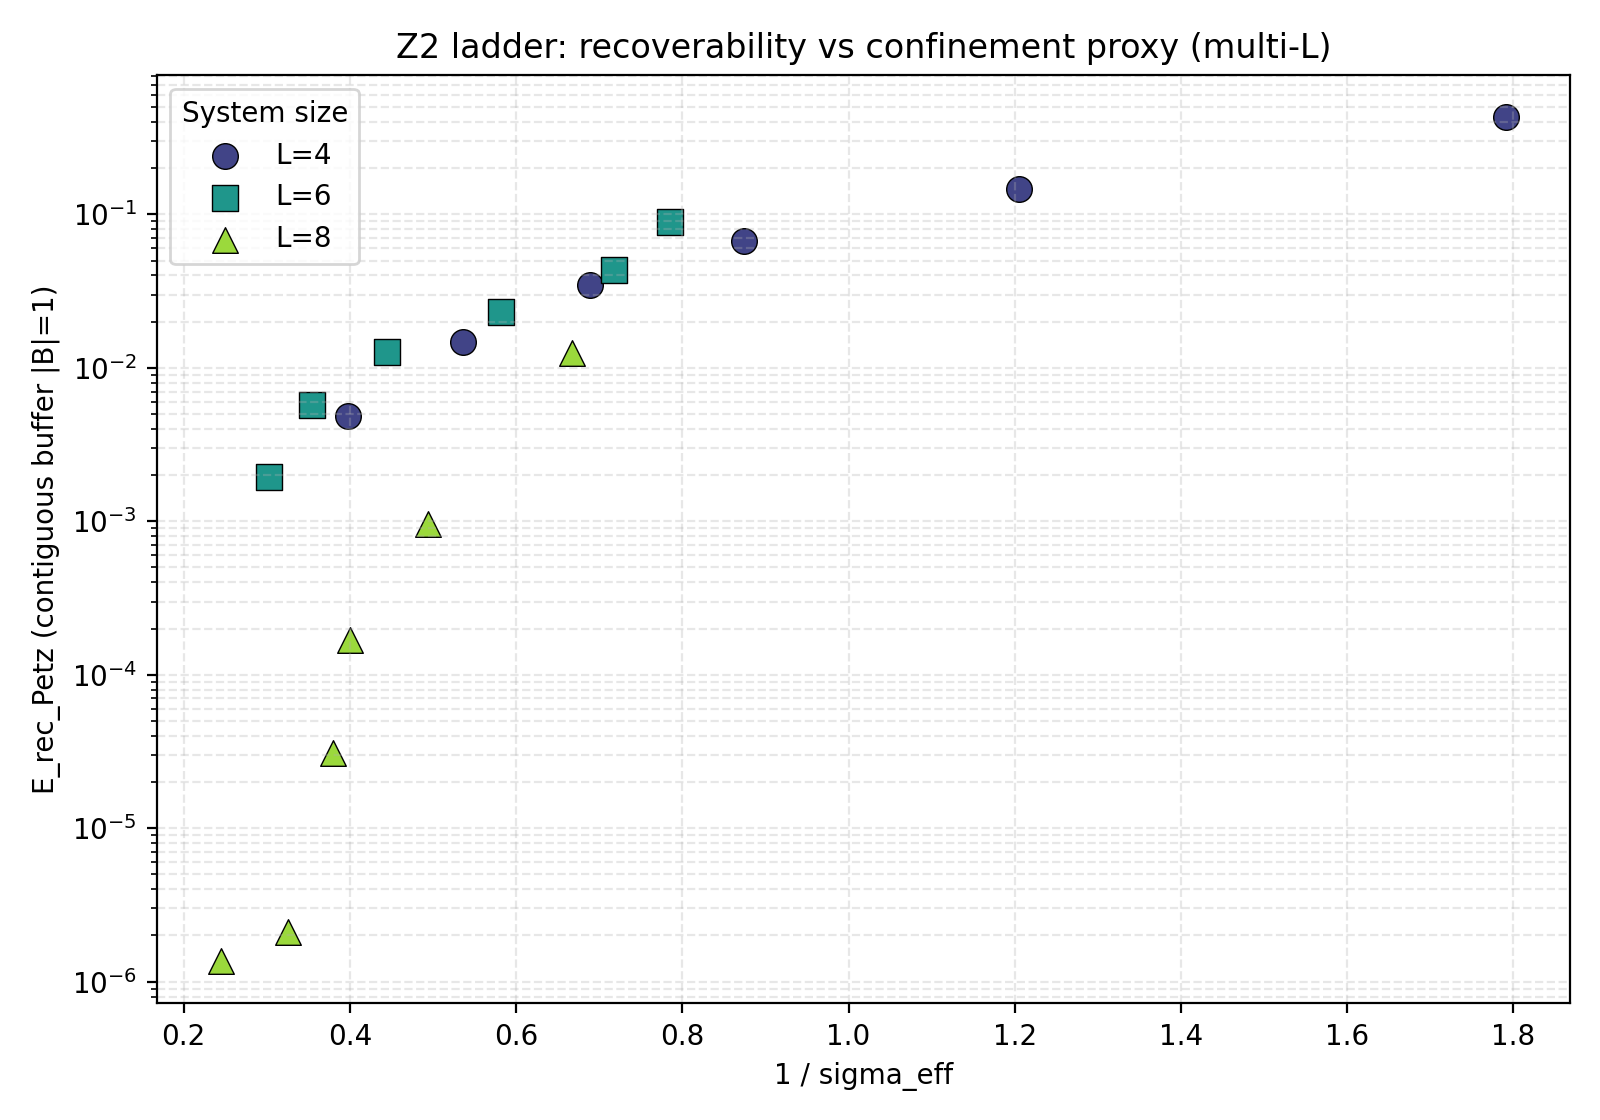
\includegraphics[width=0.45\textwidth]{fig4.png}
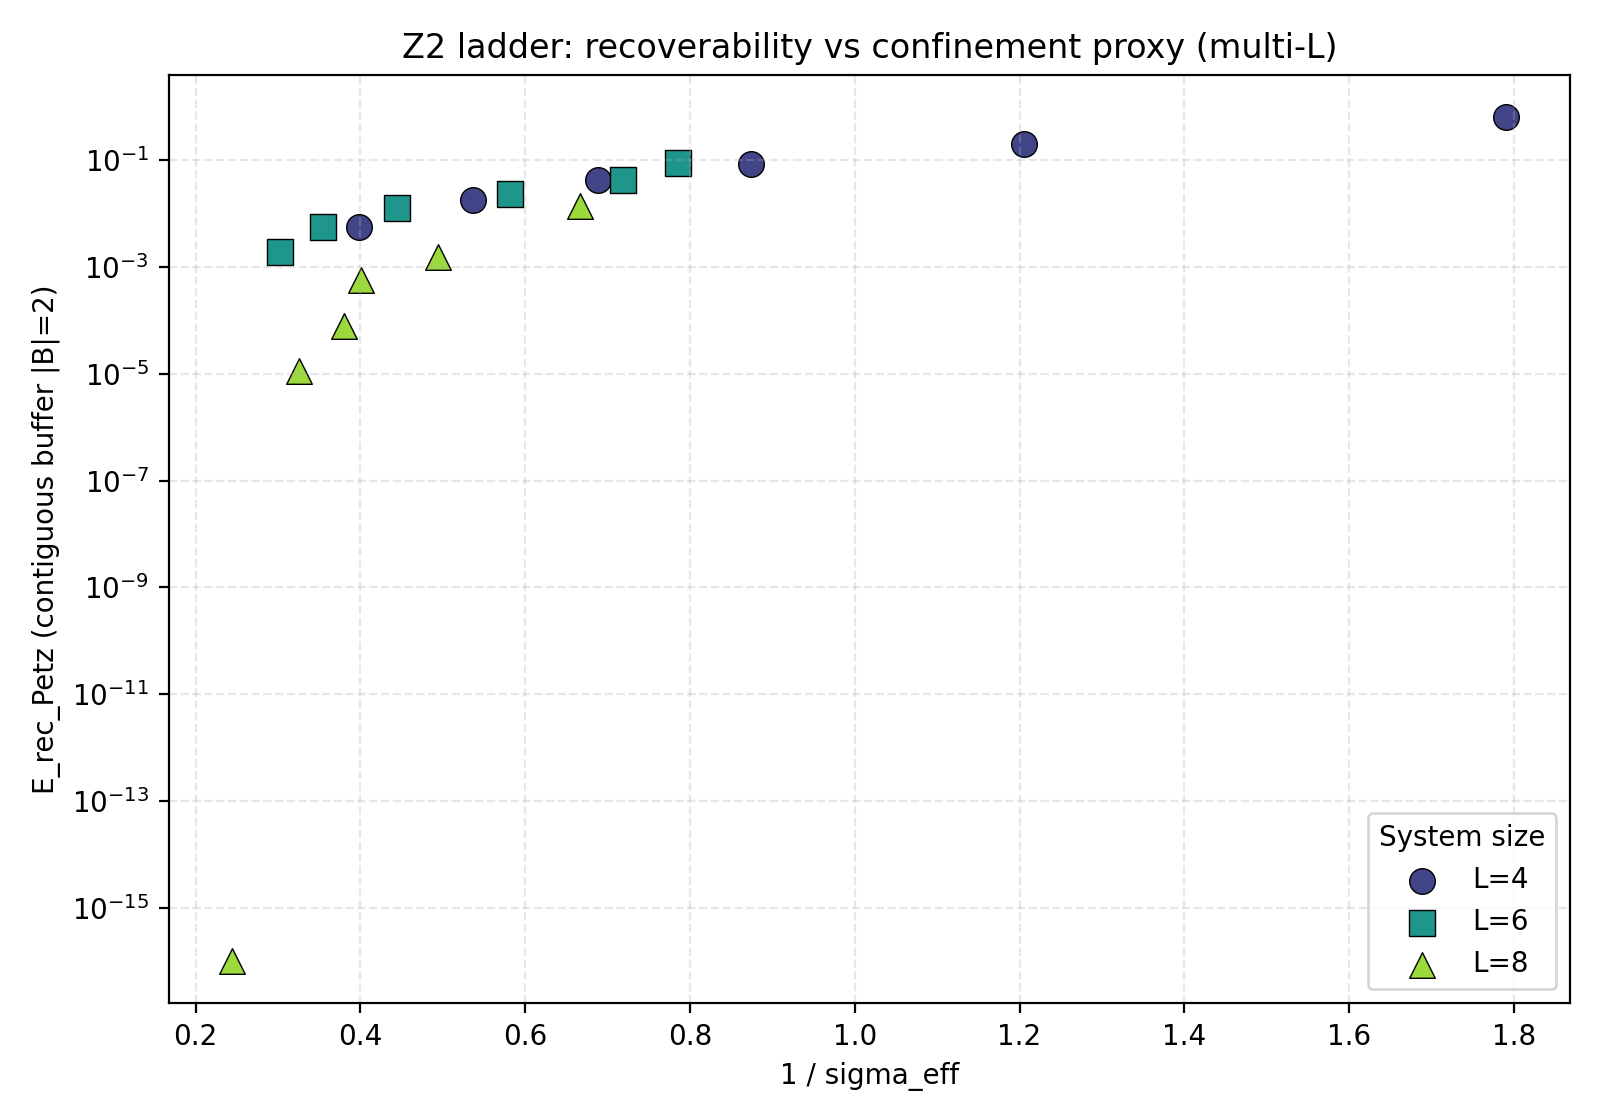
\includegraphics[width=0.45\textwidth]{fig5.png}
\caption{TN ladders (v1 figures, unchanged): fixed contiguous buffer
$|B| = 1, 2$ (MPS-ordering proxy) vs $1/\sigma_{\rm eff}$, colored by
$L$. Read with Remark~\ref{rem:proxy}.}
\end{figure}
\begin{figure}[h]\centering
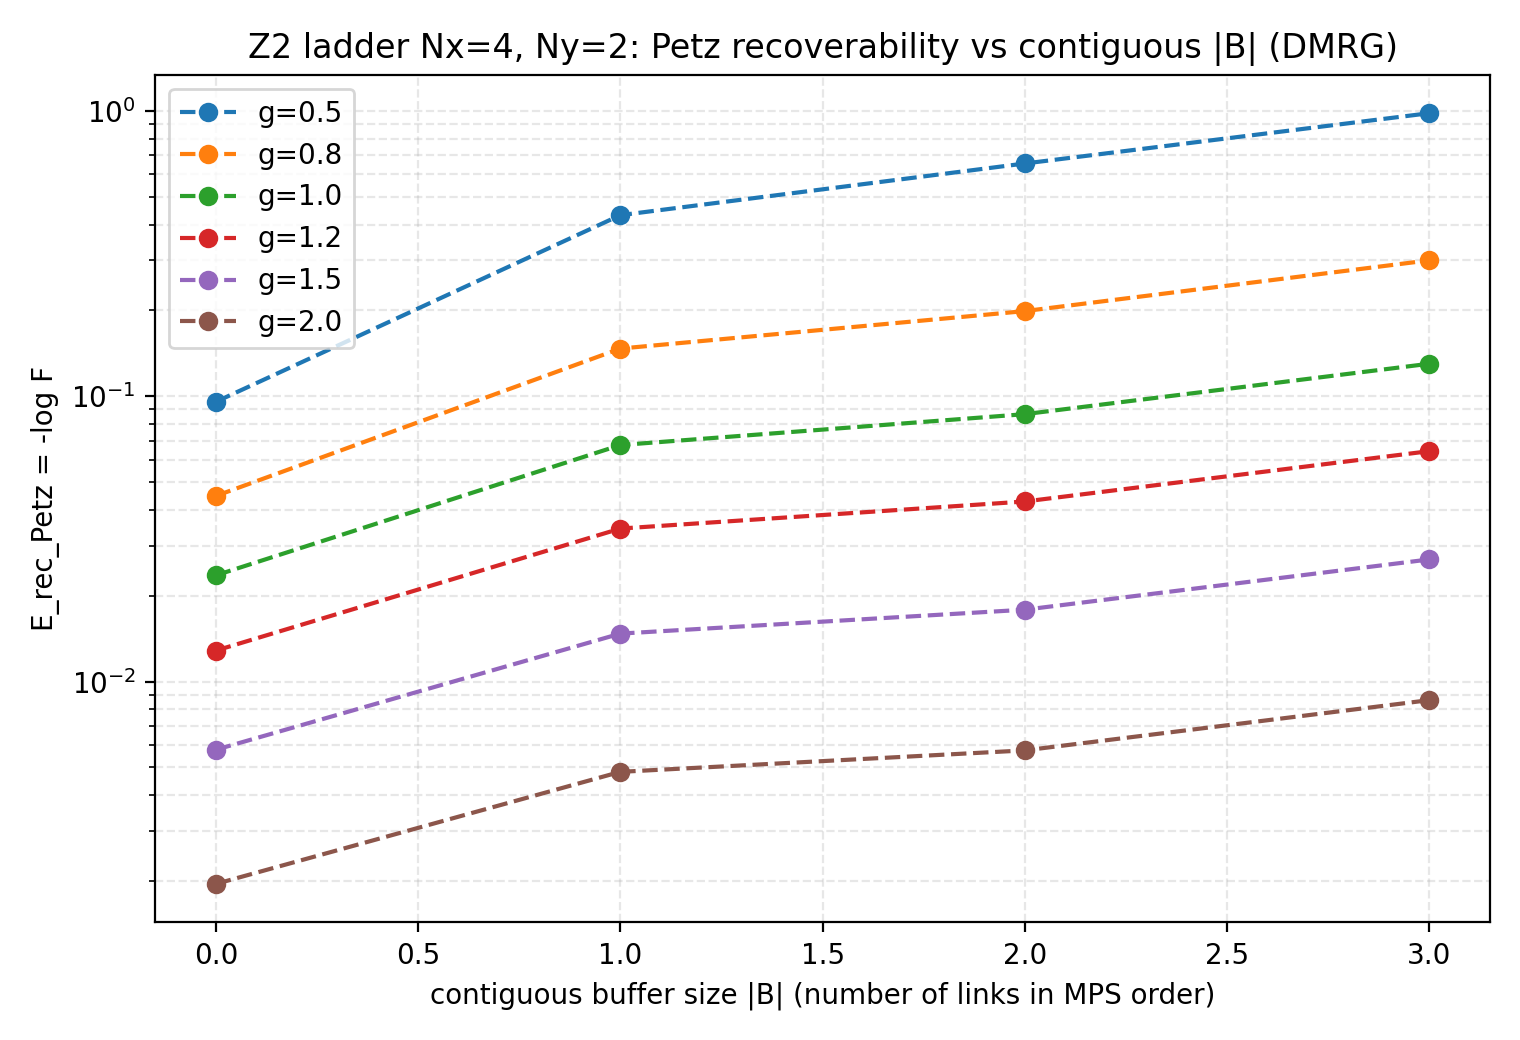
\includegraphics[width=0.32\textwidth]{fig6.png}
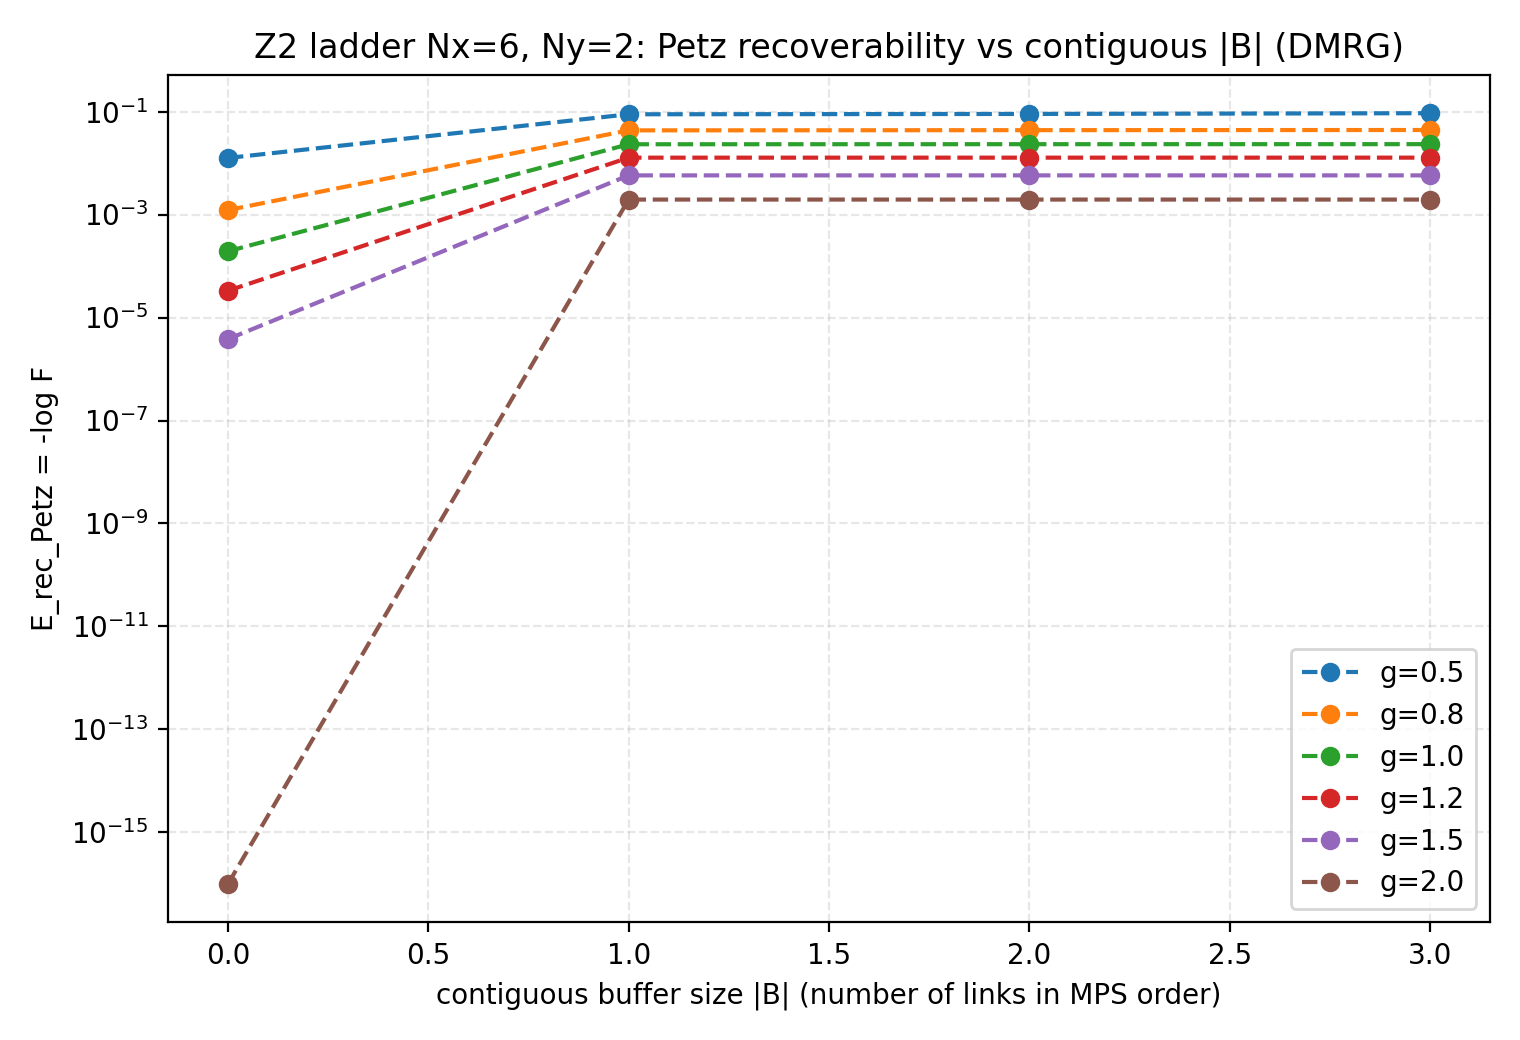
\includegraphics[width=0.32\textwidth]{fig7.png}
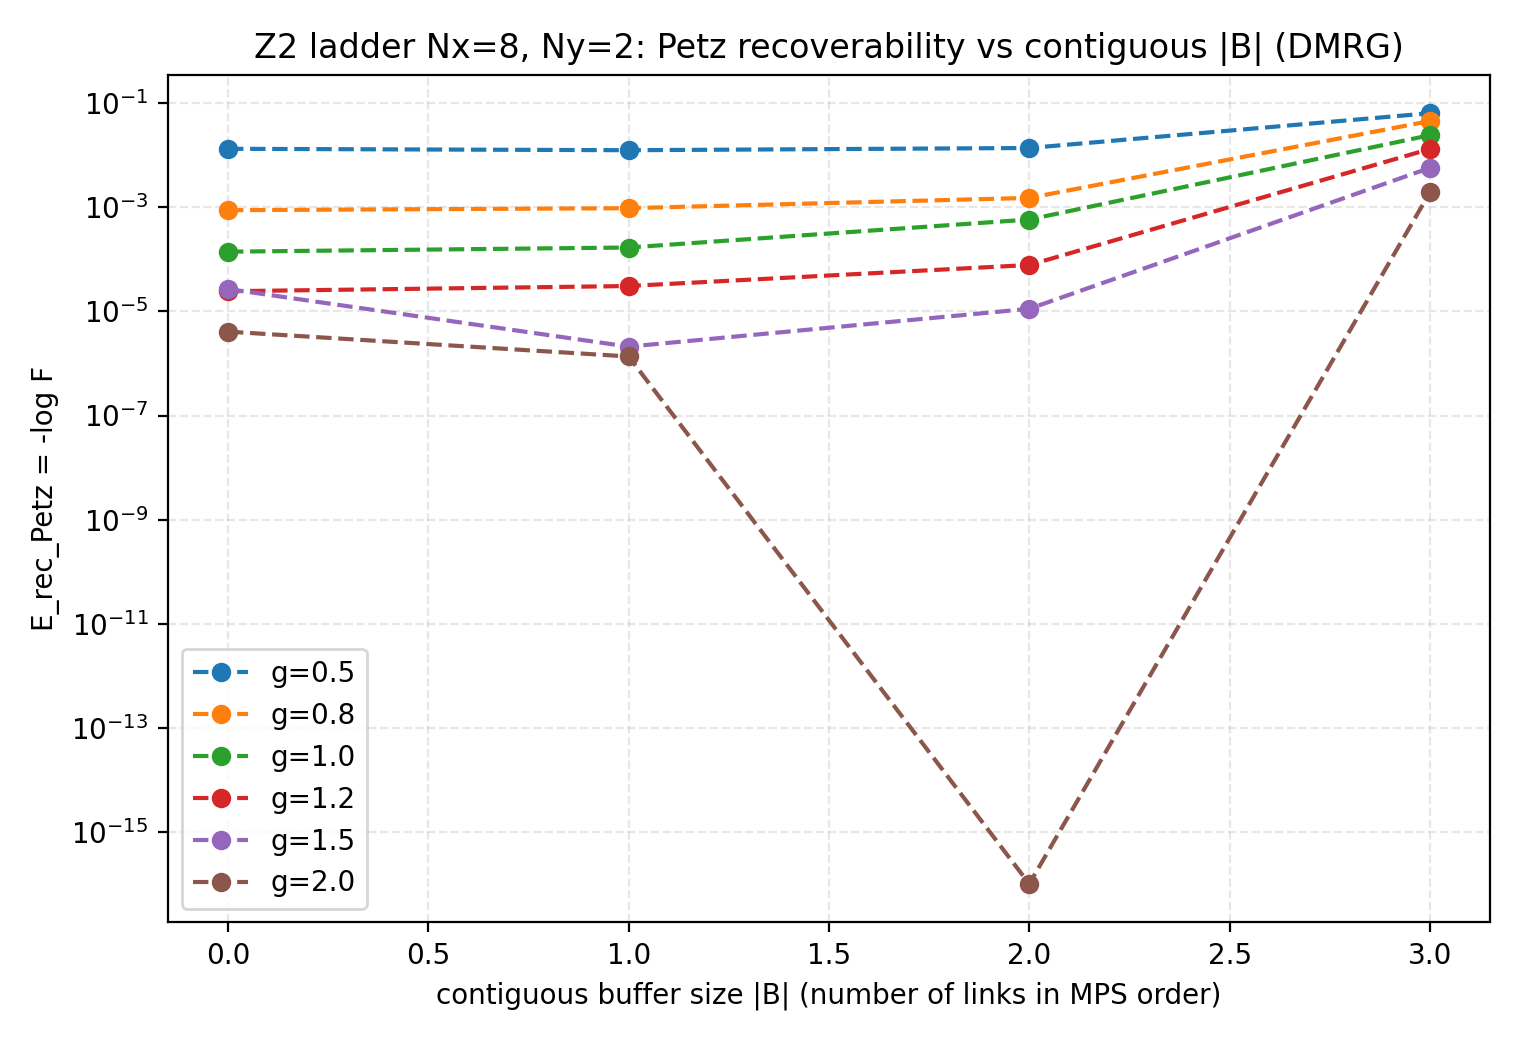
\includegraphics[width=0.32\textwidth]{fig8.png}
\caption{Recoverability profiles $\Erec(|B|)$ on ladders $2\times L$,
$L = 4, 6, 8$ (v1 figures, unchanged).}
\end{figure}

\section{Verification suite (added in v2)}
\texttt{verification/2601-0051/verify\_2601\_0051.py}: Part A
(dependency-free) runs the exact-ladder collar-semantics comparison of
Remark~\ref{rem:proxy}(i); Part B (requires TeNPy, skipped gracefully
otherwise) runs the reduced-cost DMRG replication of
Remark~\ref{rem:proxy}(ii) with Gauss checks and trend-direction
verification. The v1 TN scripts (multi-$L$ scan, validator, warm-start
check) are retained alongside, with internal working titles removed from
headers; the ED script lives with 2601.0047.

\section{Discussion}
The two-tier benchmark stands: ED with strict Gauss checks, TN ladders
with a solid bond-dimension stability check, and consistent money-plot
trends. v2's contribution is to close the reproducibility hole, quantify
what the contiguous proxy does and does not measure, and inherit the
specificity caveat of the twin. Next steps: geometric BFS collars in the
TN part, larger widths, and fixed-coupling geometry sweeps to break the
$\sigma$--gap degeneracy.

\section*{Note added in v2}
No v1 number is changed; all figures, Table 2 and the TN scripts stand.
v2: (1) repairs Appendix A.1 (the published v1 PDF prints ``Missing
file'' for the ED script; it now points to the repository, where the
script and a full ED suite live with 2601.0047); (2) removes internal
working titles leaked in v1's script headers, captions and filenames
(the historical output filenames are kept for artifact compatibility);
(3) adds the collar-semantics evidence and the DMRG replication of the
buffer inversion (Remark~\ref{rem:proxy}); (4) states the
confinement-vs-gap caveat inherited from the ED twin; (5) adds series
positioning (v1 cited no companion papers) and the verification suite.
\emph{Correction during integration review:} the exact-ladder builder in
Part A of the suite inherited an off-by-one from the 2601.0044 suite
($\texttt{NL} = 14$ instead of $13$ links for the $P = 4$ ladder),
leaving one qubit untouched by the Hamiltonian; the ground state
factorizes and the pure spectator provably cancels in all reported
quantities. Fixed to $\texttt{NL} = 13$ and regenerated: all Part-A
conclusions are unchanged (floor-level jitter only).

\begin{thebibliography}{10}
\bibitem{Kogut} J. B. Kogut, Rev. Mod. Phys. \textbf{51} (1979)
659--713.
\bibitem{Petz} D. Petz, Commun. Math. Phys. \textbf{105} (1986)
123--131.
\bibitem{FR} O. Fawzi and R. Renner, Commun. Math. Phys. \textbf{340}
(2015) 575--611.
\bibitem{Donnelly} W. Donnelly, Phys. Rev. D \textbf{85} (2012) 085004.
\bibitem{CHR} H. Casini, M. Huerta, and J. A. Rosabal, Phys. Rev. D
\textbf{89} (2014) 085012.
\bibitem{TeNPy} J. Hauschild and F. Pollmann, SciPost Phys. Lect. Notes
5 (2018) [TeNPy].
\bibitem{S0047} L. Eriksson, ai.viXra:2601.0047 (2026; v2 2026).
\bibitem{S0050} L. Eriksson, ai.viXra:2601.0050 (2026; v2 2026).
\bibitem{S0044} L. Eriksson, ai.viXra:2601.0044 (2026; v2 2026).
\bibitem{S0043} L. Eriksson, ai.viXra:2601.0043 (2026; v2 2026).
\end{thebibliography}
\end{document}
